\chapter{Технологическая часть}

\section{Выбор СУБД}

В аналитической части выбрана реляционная модель. Для реализации рассмотрены PostgreSQL, MySQL и SQLite. Сравнение по требованиям проекта приведено в таблице~\ref{tab:technology-dbms}. PostgreSQL предоставляет ограничения связей, транзакции, триггеры и права на объекты БД~\cite{postgresql-features,postgresql-privileges}. MySQL также поддерживает перечисленные механизмы~\cite{mysql-privileges,mysql-transactions}. SQLite поддерживает триггеры и транзакции~\cite{sqlite-triggers,sqlite-transactions}; внешние ключи включаются отдельно для каждого соединения, а разграничение доступа командами \texttt{GRANT} и \texttt{REVOKE} отсутствует~\cite{sqlite-foreign-keys,sqlite-omitted}.

\begin{table}[H]
    \caption{Сравнение СУБД по требованиям проекта}
    \label{tab:technology-dbms}
    \small
    \begin{tabularx}{\textwidth}{|p{5.1cm}|Y|Y|Y|}
        \hline
        \textbf{Критерий} & \textbf{PostgreSQL} & \textbf{MySQL} & \textbf{SQLite} \\
        \hline
        Внешние ключи & Да & Да & Да, после включения \\
        \hline
        Транзакции & Да & Да & Да \\
        \hline
        Триггеры для строк & Да & Да & Да \\
        \hline
        Роли и права на таблицы & Да & Да & Нет \\
        \hline
    \end{tabularx}
\end{table}

Для JoinUp выбрана PostgreSQL~16: она позволяет реализовать таблицы, триггер и три роли подключений средствами одной СУБД. MySQL также отвечает этим требованиям. Выбор PostgreSQL согласуется с примененным в проекте драйвером \texttt{pgx} и существующими SQL-миграциями.

\section{Средства реализации}

Сервер написан на Go~1.25. Для маршрутизации HTTP-запросов используется Echo~5, для доступа к PostgreSQL -- \texttt{pgx/v5}, для применения SQL-миграций -- Goose~3. Клиентская часть написана на React~18 и TypeScript; сборку выполняет Vite. Версии взяты из \texttt{app/go.mod} и \texttt{frontend/package.json}.

HTTP-сервер принимает запросы по маршрутам \texttt{/api/v1}, проверяет данные и вызывает сервисы. Сервисы проверяют правила приложения, а репозитории выполняют SQL-запросы. Схема взаимодействия показана на рисунке~\ref{fig:design-architecture}. Доступ к операциям с мероприятиями и профилем определяется токеном пользователя; подключение сервера к БД выполняется под ролью \texttt{joinup\_user}. Роли приложения и роли подключений не совпадают.

\section{Реализация базы данных}

Миграции выполняются Goose в порядке имен файлов: создание основных таблиц, категорий и уникальности участия, отзывов, журнала удаления, индекса поиска и прав ролей. Команда \texttt{make migrate\_up} применяет их через \texttt{app/cmd/migrations}. Структура всех~11~таблиц и связи уже приведены в конструкторской части; здесь рассматриваются конкретные средства PostgreSQL.

Идентификаторы основных таблиц созданы типом \texttt{serial}; у \texttt{review} и \texttt{event\_deletion\_log} используется \texttt{bigserial}. Для названий и описаний применен \texttt{text}, для времени -- \texttt{timestamp}, для признака удаления -- \texttt{boolean}, для изображения -- \texttt{bytea}, для координат -- \texttt{float}. Внешние ключи связывают мероприятие с автором и локацией, отзыв -- с мероприятием и автором. Ограничение \texttt{UNIQUE} установлено для пары мероприятие/автор отзыва; уникальный индекс -- для пары пользователь/мероприятие в \texttt{member}. Оценка ограничена значениями от~1 до~5, длина текста отзыва -- 2000~символами. Проверка непустого текста после удаления пробелов выполняется в сервисе.

Для поиска создан частичный индекс \texttt{event\_search\_city\_date\_idx} по полям \texttt{city}, \texttt{event\_date}, \texttt{id} при \texttt{deleted = false}. Он соответствует фильтрации по городу и диапазону времени; исследование его влияния приведено в исследовательской части.

Функция \texttt{log\_event\_deletion} вызывается построчным триггером после обновления поля \texttt{deleted} в \texttt{event}. Существенный фрагмент реализации:

\begin{verbatim}
if old.deleted = false and new.deleted = true then
    insert into event_deletion_log (event_id) values (new.id);
end if;
\end{verbatim}

Алгоритм показан на рисунке~\ref{fig:deletion-algorithm}. При повторной установке признака удаления запись в журнал не добавляется. Вставка в журнал и исходное обновление выполняются атомарно в рамках одного SQL-оператора.

Миграция ролей создает \texttt{joinup\_guest}, \texttt{joinup\_user} и \texttt{joinup\_admin}, затем выдает права на схему, таблицы и последовательности. Например, гостю разрешено чтение мероприятий, локаций, изображений, категорий и отзывов:

\begin{verbatim}
grant select on event, location, image, category,
    event_category, review to joinup_guest;
\end{verbatim}

Полная матрица прав представлена в таблице~\ref{tab:design-roles}. Роль \texttt{joinup\_user} имеет право записи в журнал, которое требуется функции триггера; она может изменять журнал и напрямую. При авторизации в приложении роль подключения не переключается. SQL-сценарий создания объектов БД приведен в приложении~А.

\section{Доступ к данным и запросы}

Репозитории используют пул соединений \texttt{pgxpool.Pool}. Значения фильтров и изменяемых полей передаются параметрами \texttt{\$1}, \texttt{\$2} и~т.~д. Объект управления транзакцией передается через контекст операции; репозиторий выбирает транзакцию из контекста или пул соединений. Создание мероприятия, загрузка его обложки и создание отзыва используют явные транзакции, перечисленные в таблице~\ref{tab:design-transactions}.

Поиск выполняется методом \texttt{SearchEvents}. Запрос исключает удаленные объявления, соединяет \texttt{event} с \texttt{location}, применяет фильтры названия, дат и города. Для выбора мероприятий, содержащих все указанные категории, применяется подзапрос с группировкой по мероприятию и условием \texttt{HAVING COUNT(DISTINCT category\_id)}. Результаты упорядочиваются по времени и идентификатору. После основного запроса сведения об авторах, участниках и категориях загружаются отдельными запросами.

Соответствие запросов приложения основным видам SQL приведено в таблице~\ref{tab:technology-queries}.

\begin{table}[H]
    \caption{Виды запросов в репозиториях PostgreSQL}
    \label{tab:technology-queries}
    \small
    \begin{tabularx}{\textwidth}{|p{3.7cm}|X|}
        \hline
        \textbf{Вид запроса} & \textbf{Пример применения} \\
        \hline
        Простой & Чтение пользователя по логину из \texttt{users} \\
        \hline
        Многотабличный & Поиск мероприятий с присоединением \texttt{location} \\
        \hline
        Агрегатный & Средняя оценка организатора через \texttt{AVG} \\
        \hline
        С группировкой & Подбор мероприятий по всем выбранным категориям \\
        \hline
        С подзапросом & Подсчет отзывов о мероприятиях организатора в \texttt{GetUser} \\
        \hline
        Изменение данных & Добавление мероприятия и обновление признака удаления \\
        \hline
    \end{tabularx}
\end{table}

Рейтинг организатора не хранится отдельным полем: метод \texttt{GetUser} получает его из отзывов агрегатной функцией \texttt{AVG}.

\section{Интерфейс и подготовка данных}

В клиентском приложении имеются экраны регистрации, входа, поиска, созданных мероприятий, участий, профиля и карточки мероприятия. Поиск с заданными фильтрами показан на рисунке~\ref{fig:ui-search}. В карточке мероприятия (рисунок~\ref{fig:ui-event}) видны описание, место проведения, карта и ссылка на чат. Пользователь может присоединиться к мероприятию, автор -- изменить или удалить его. Изображения загружаются через сервер; для выбора адреса и отображения карты используются API Яндекса при наличии настроенных ключей.

\begin{figure}[H]
    \centering
    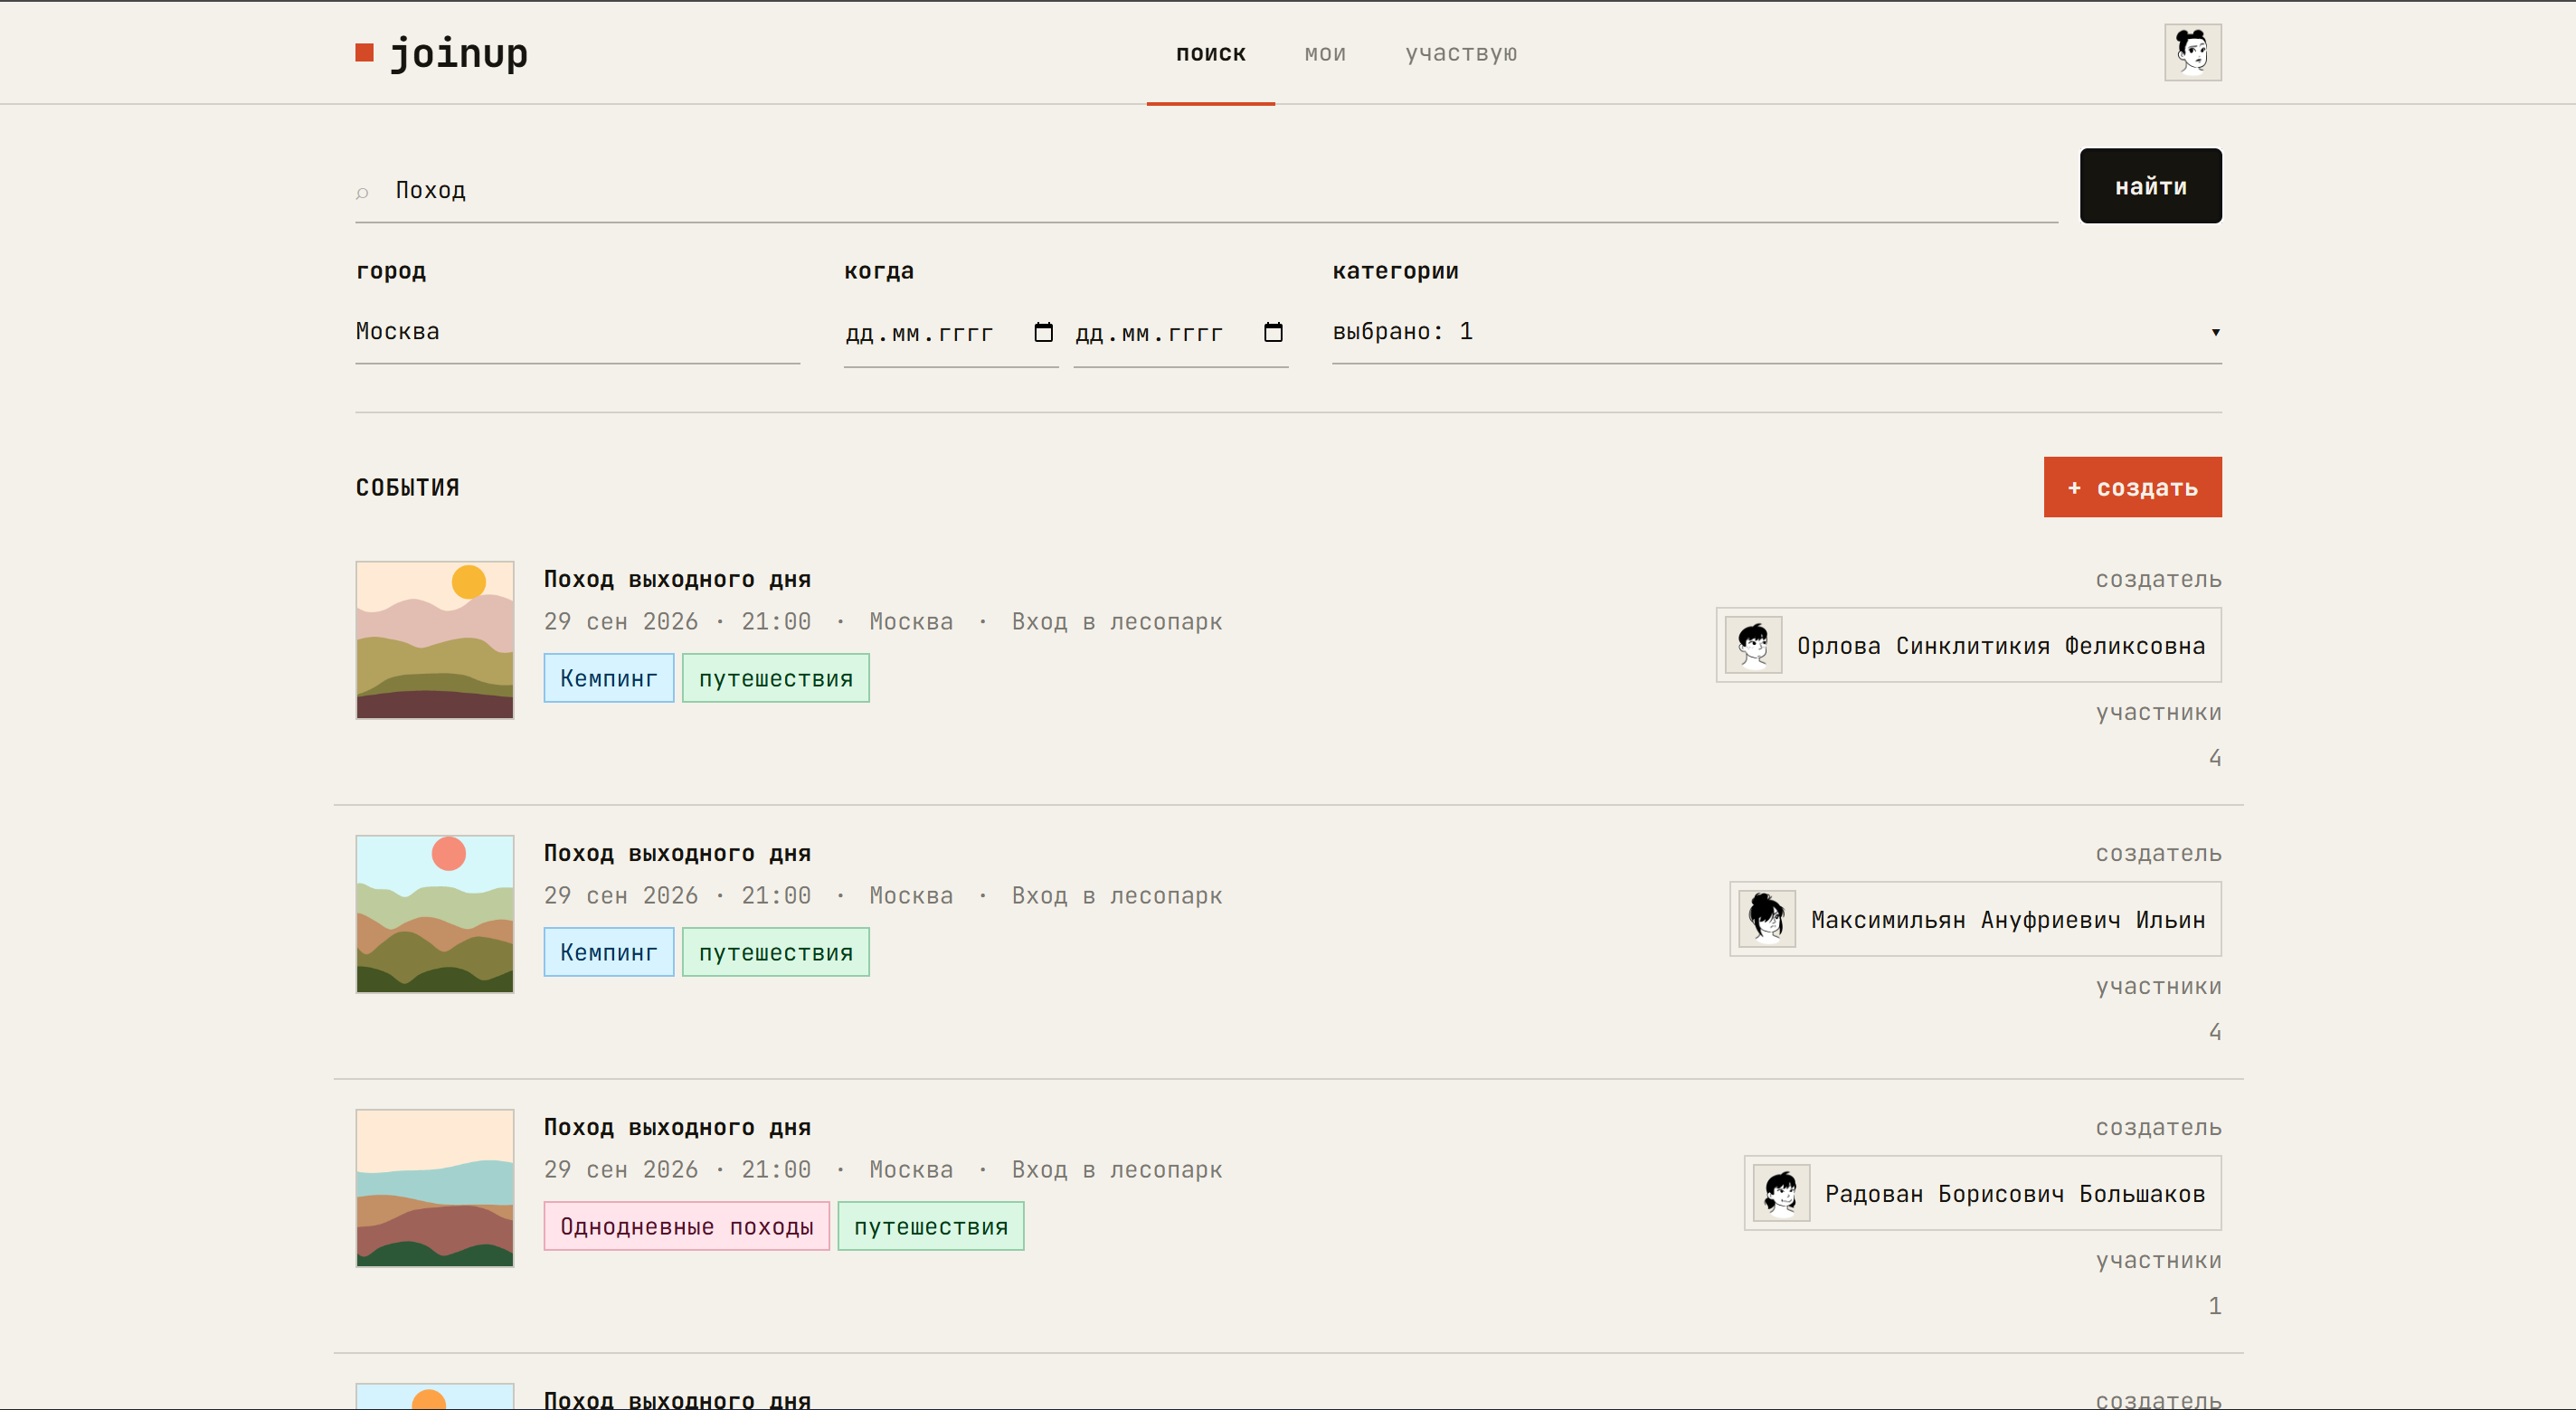
\includegraphics[width=\textwidth]{ui-search.png}
    \caption{Поиск мероприятий с фильтрами}
    \label{fig:ui-search}
\end{figure}

\begin{figure}[H]
    \centering
    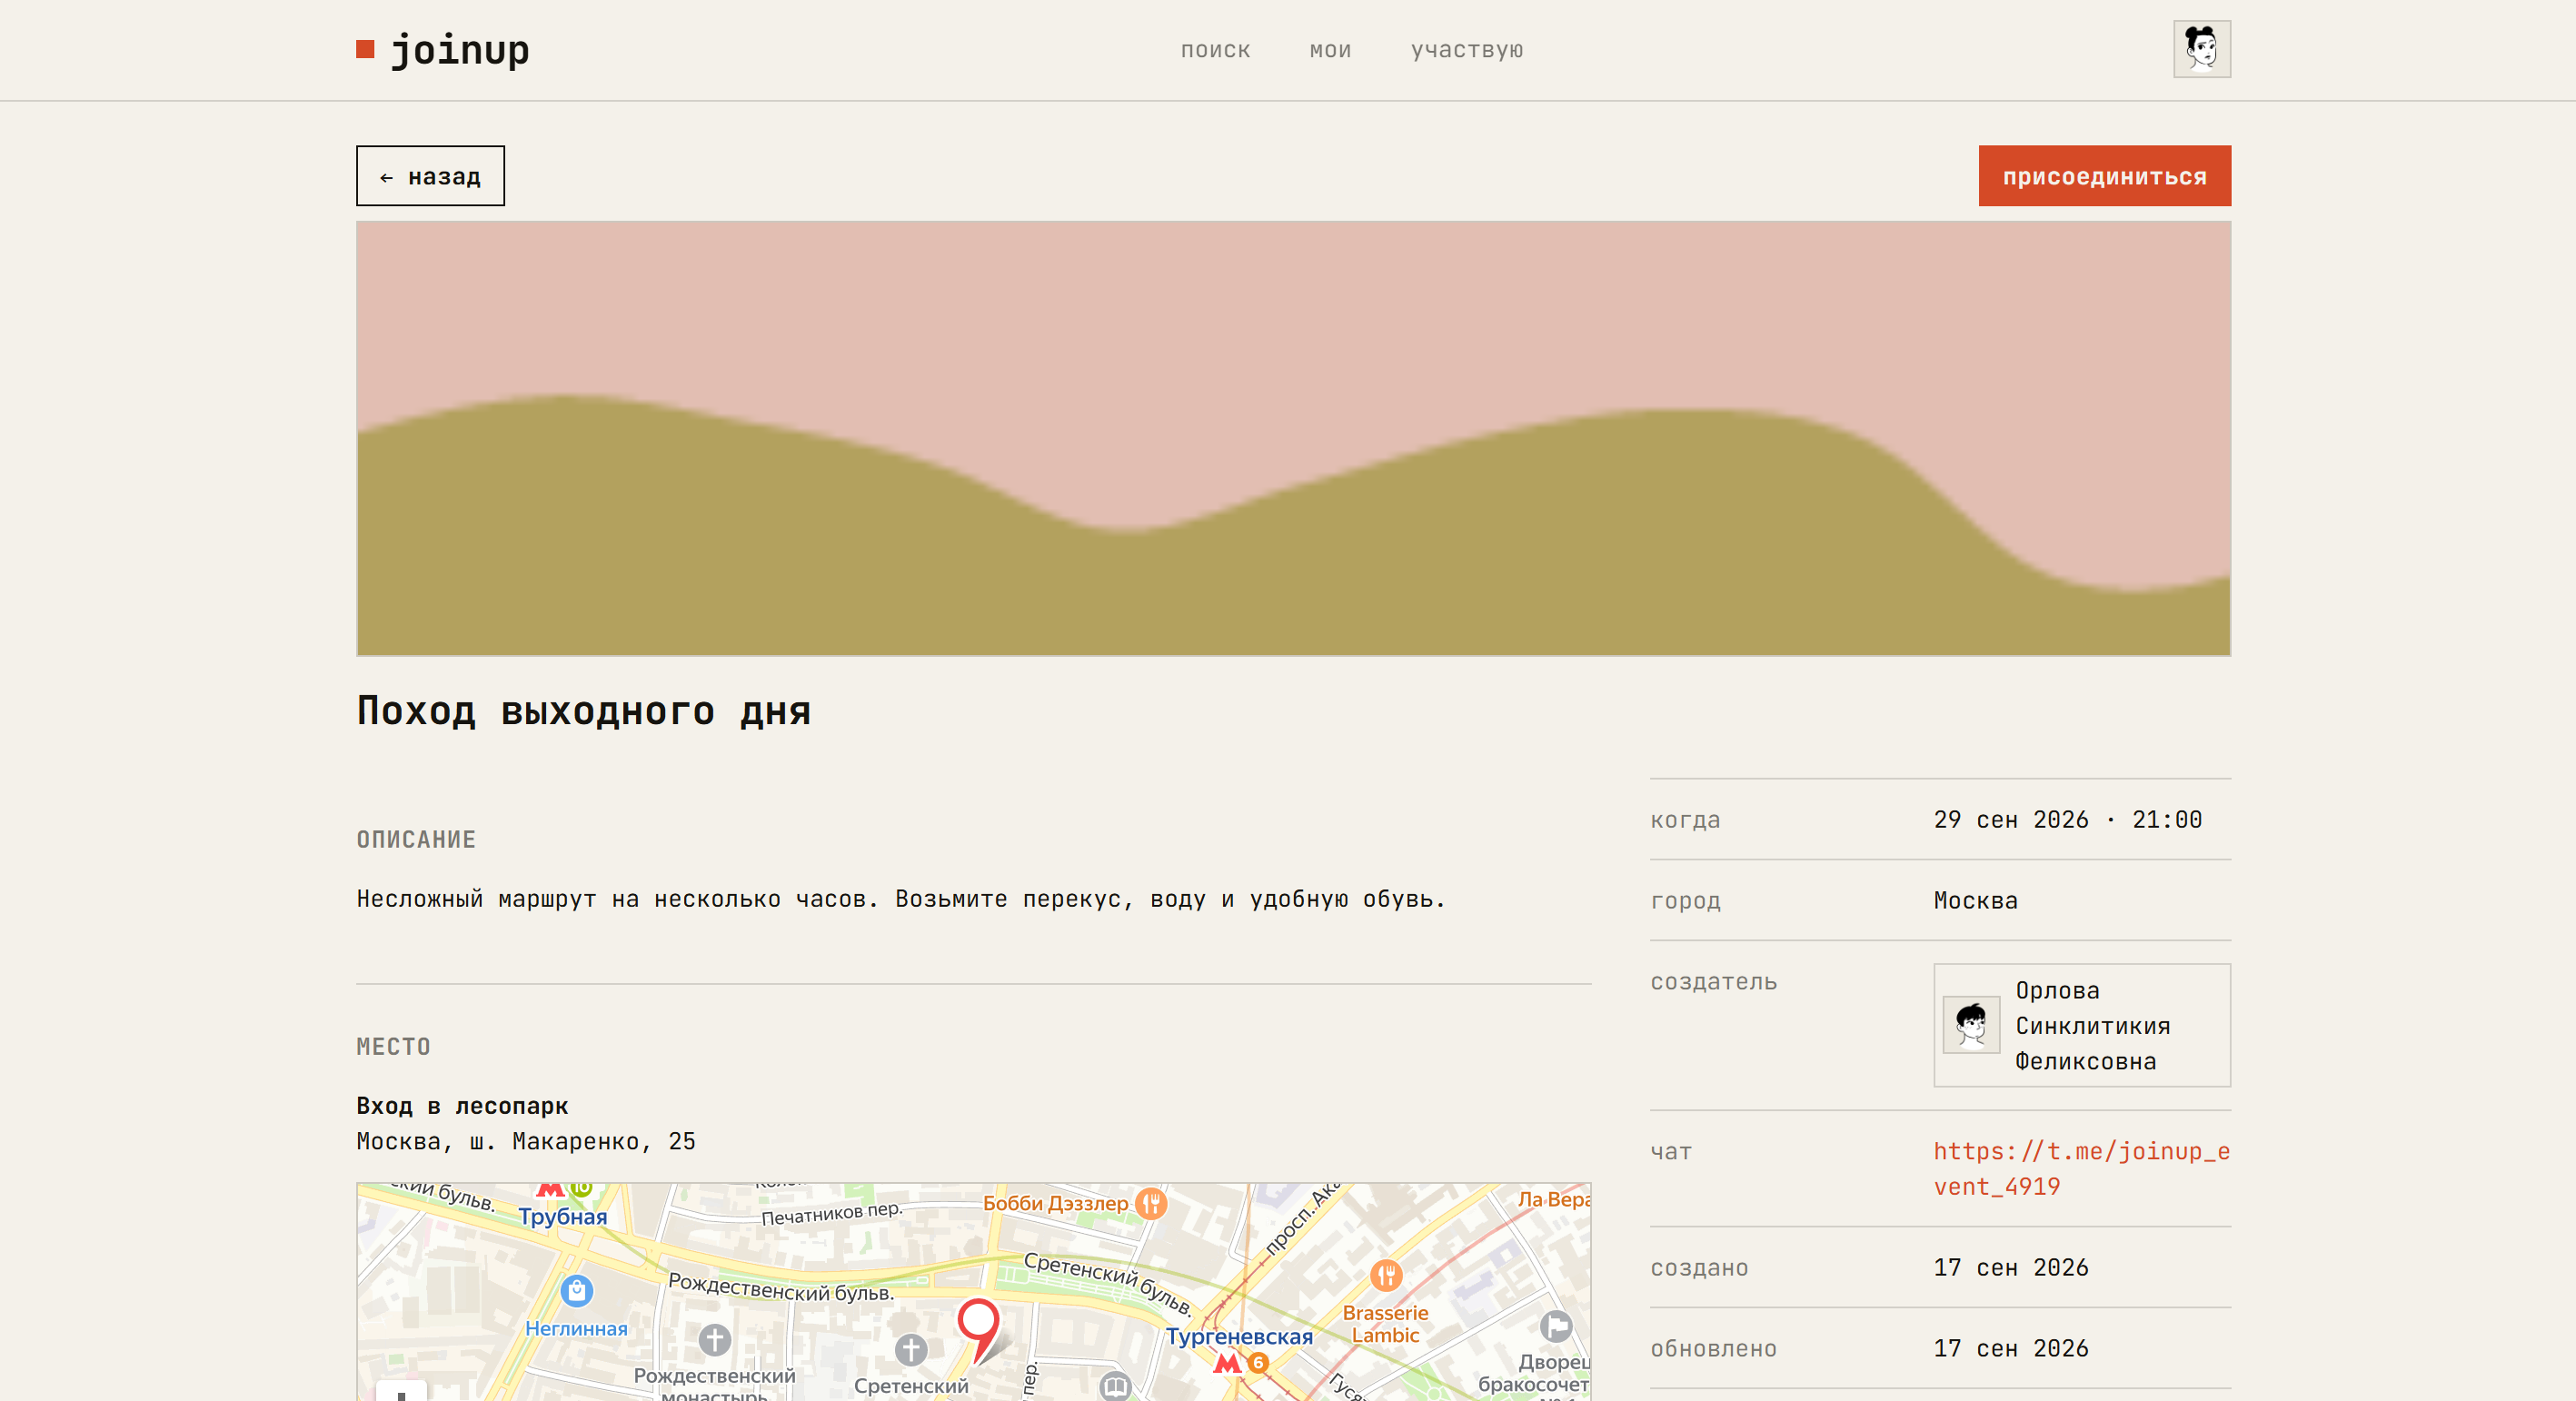
\includegraphics[width=\textwidth]{ui-event.png}
    \caption{Карточка мероприятия}
    \label{fig:ui-event}
\end{figure}

Режим редактирования мероприятия представлен на рисунке~\ref{fig:ui-edit}, профиль пользователя с показателями участия и рейтингом -- на рисунке~\ref{fig:ui-profile}.

\begin{figure}[H]
    \centering
    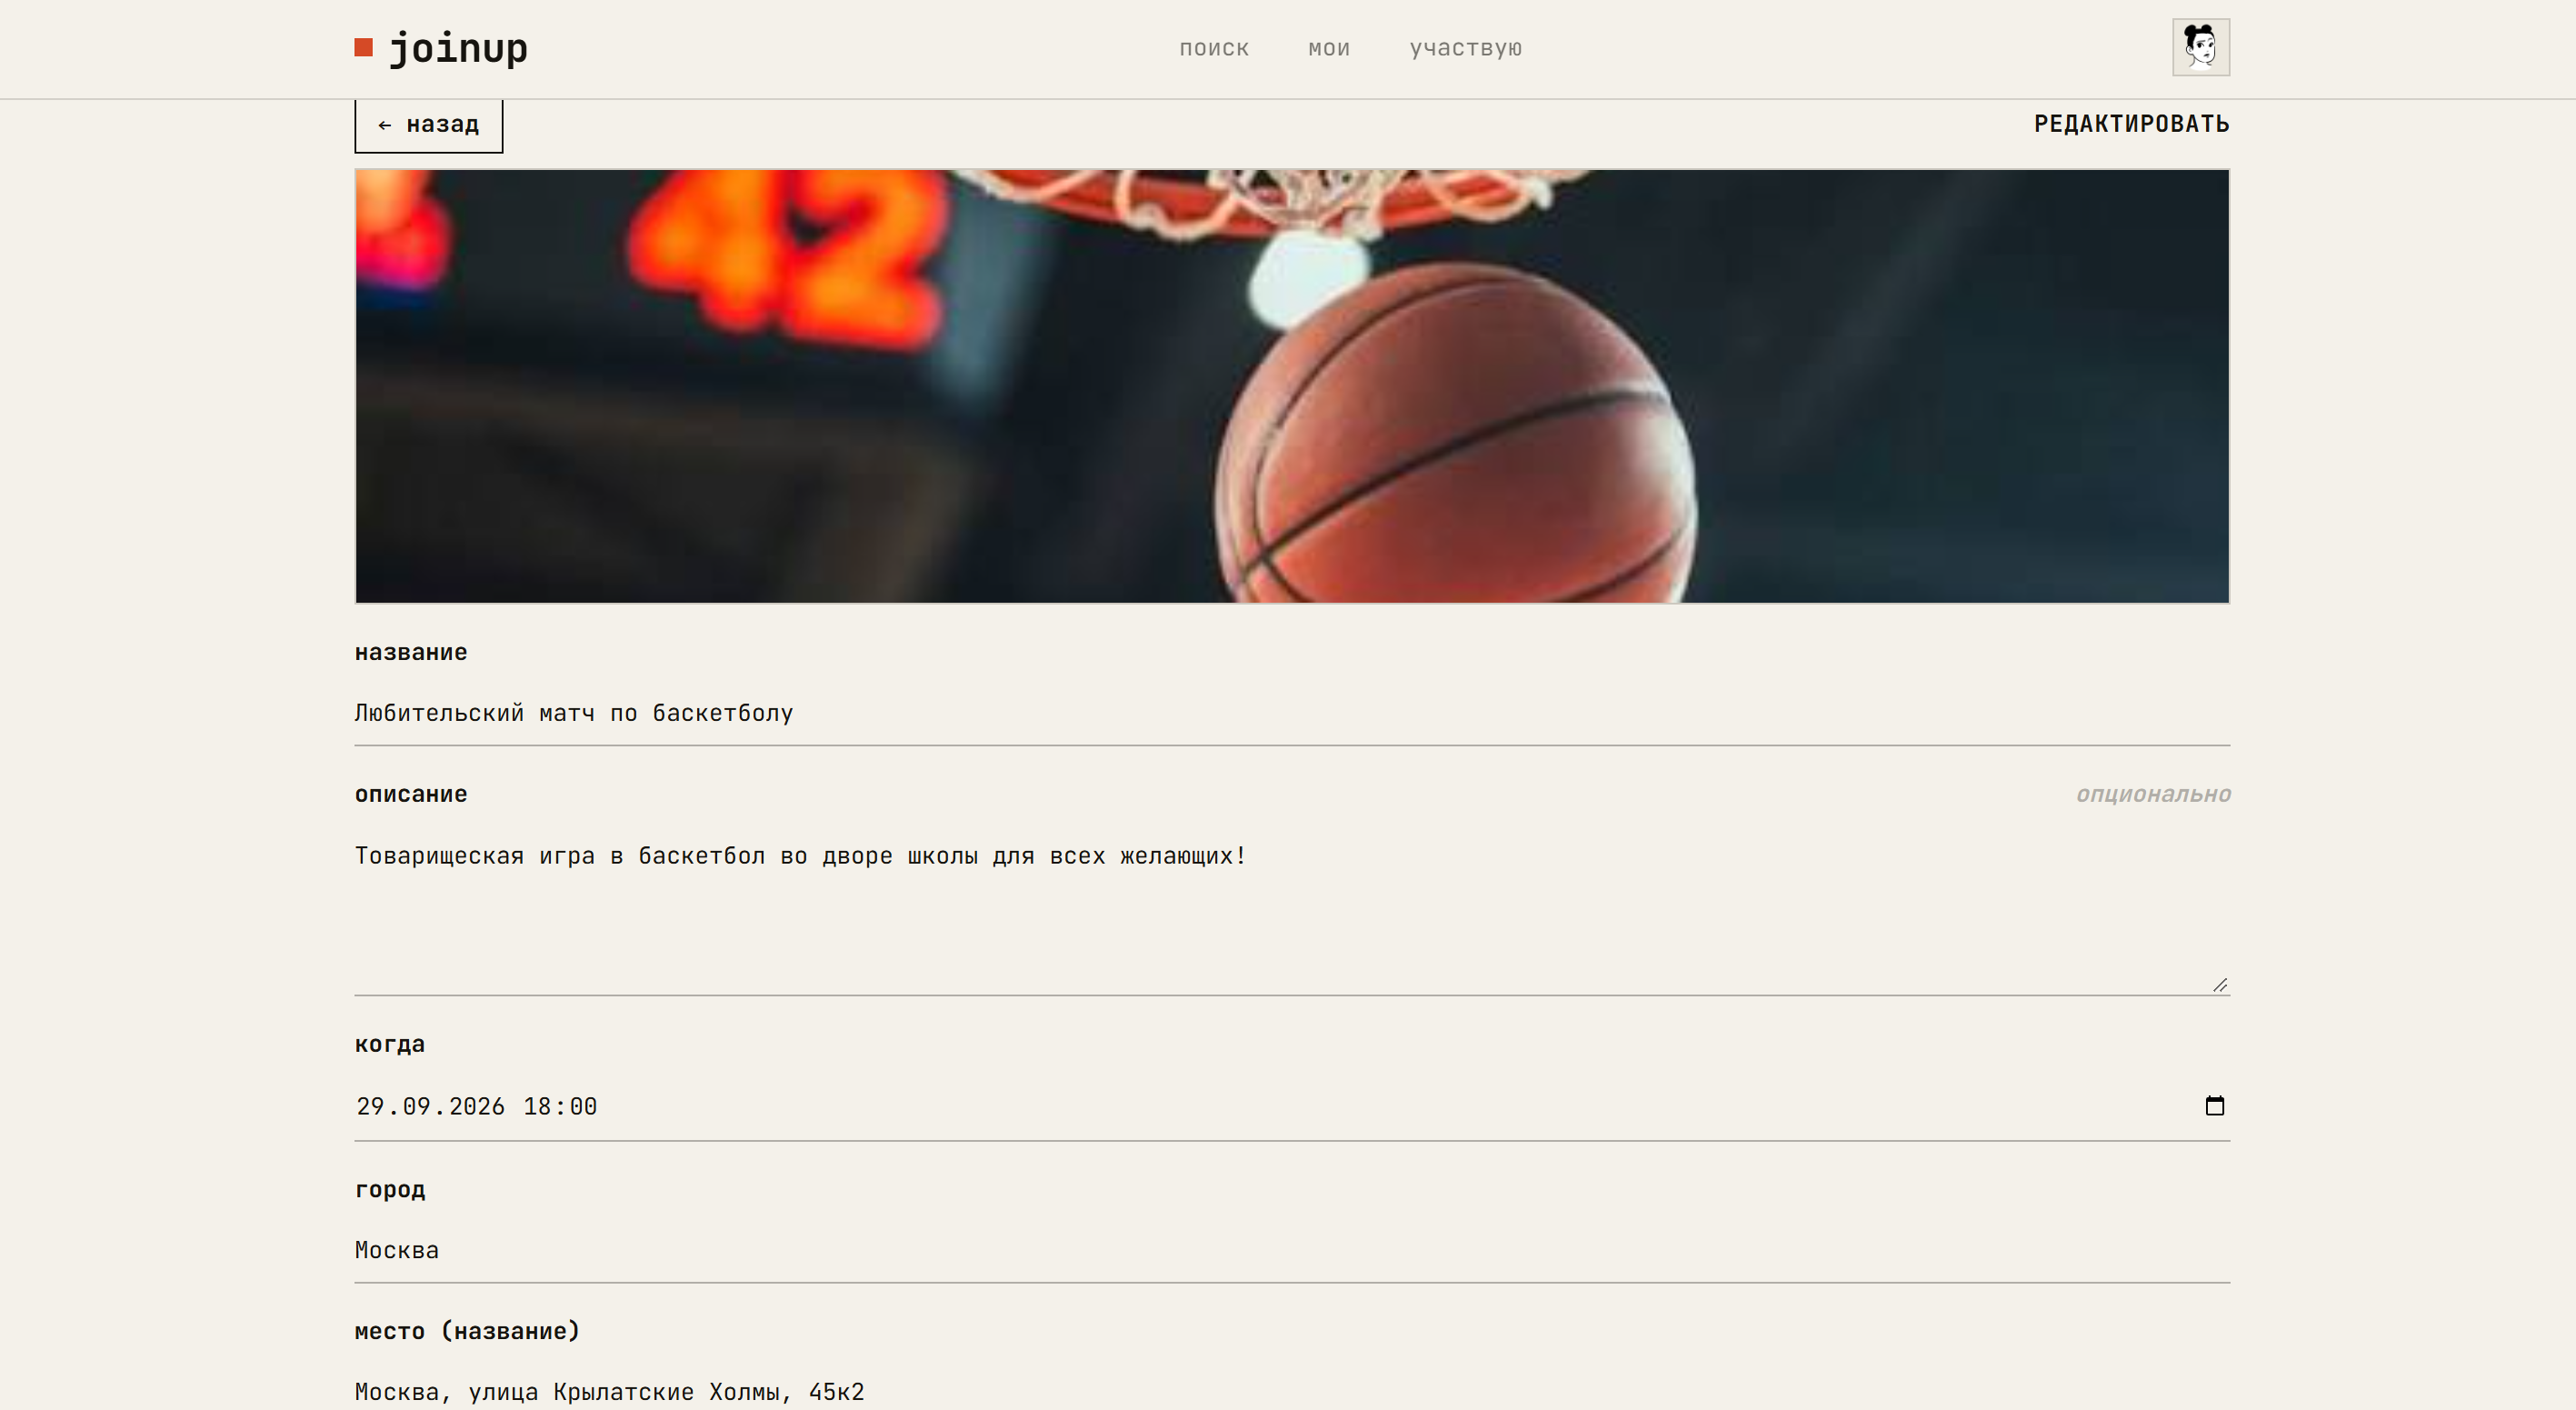
\includegraphics[width=\textwidth]{ui-create.png}
    \caption{Редактирование мероприятия}
    \label{fig:ui-edit}
\end{figure}

\begin{figure}[H]
    \centering
    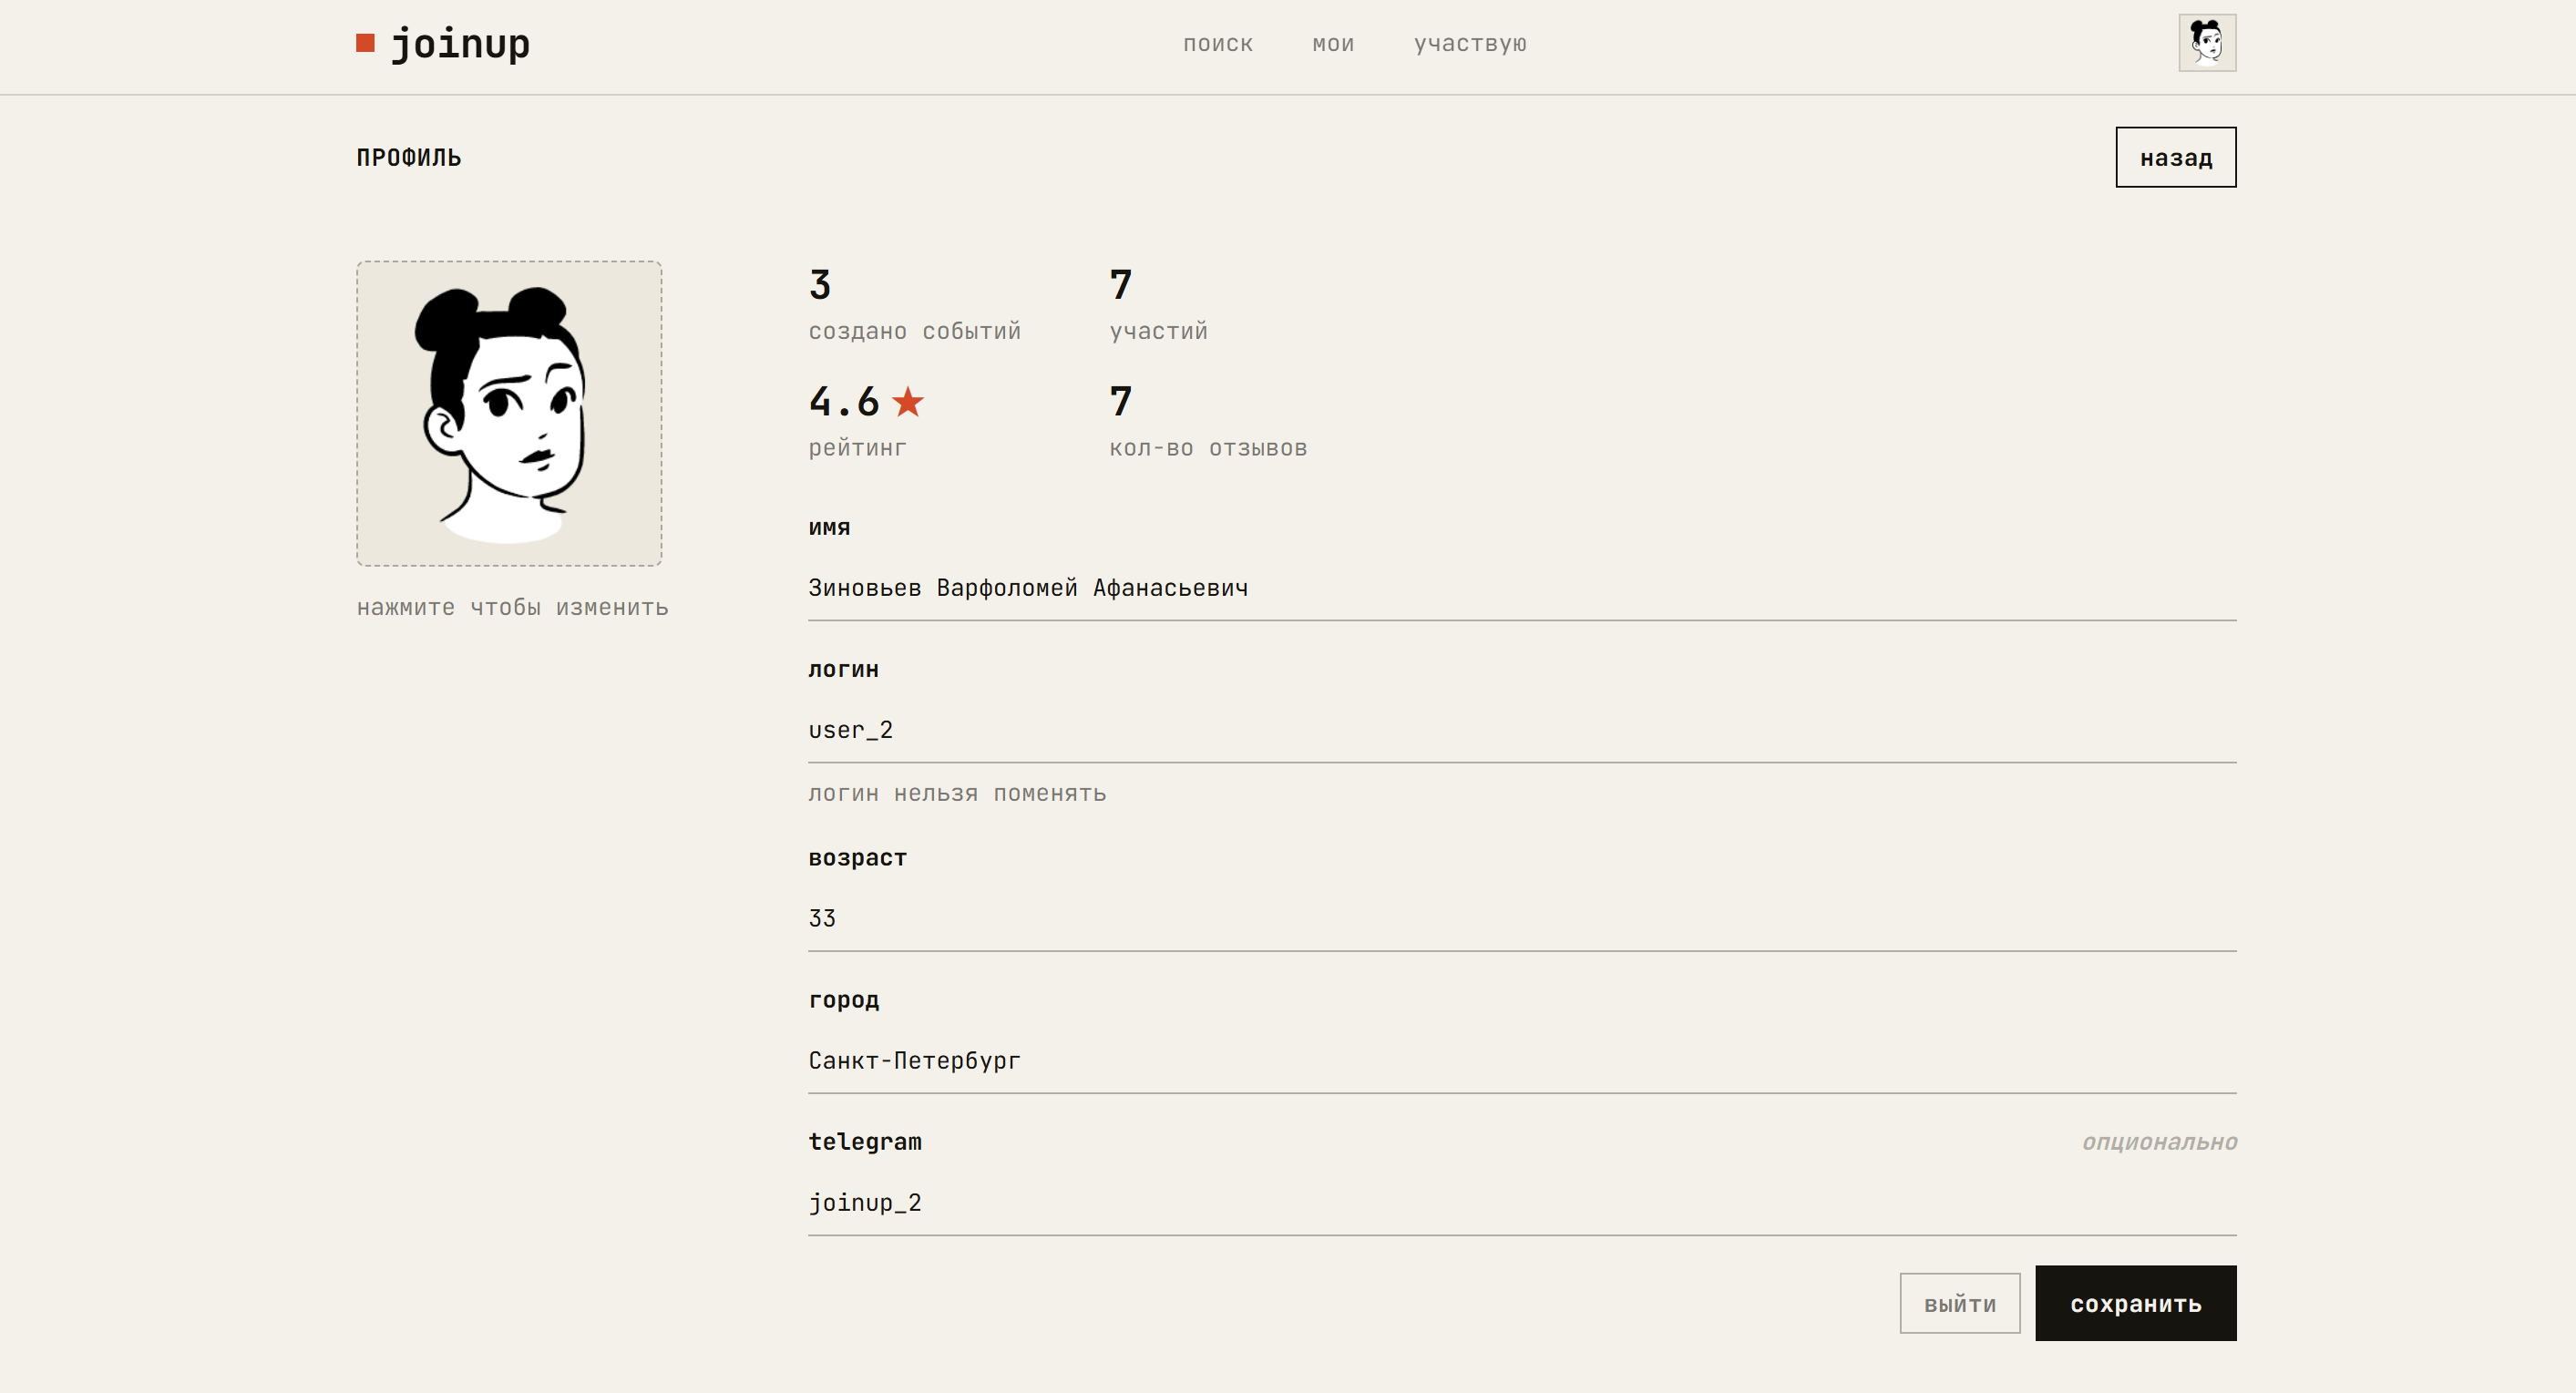
\includegraphics[width=\textwidth]{ui-profile.png}
    \caption{Профиль пользователя}
    \label{fig:ui-profile}
\end{figure}

Учебные данные формирует \texttt{app/scripts/seed.py}. Он использует Faker с локалью \texttt{ru\_RU}, справочные значения из \texttt{seed\_data.json} и Pillow для генерации PNG. Сценарий создает 5001~пользователя; каждый создает от~1 до~3~мероприятий, участвует в нескольких мероприятиях, часть пользователей оставляет отзывы. После заполнения примерно 5\% мероприятий помечаются удаленными, что вызывает триггер журнала. Затем учебные аватары и обложки были заменены изображениями DiceBear. Количества строк на 28.09.2026 приведены в таблице~\ref{tab:technology-rows}. Справочник содержит 11~направлений и по~8~конкретных тем в каждом.

\begin{table}[H]
    \caption{Количество строк в таблицах БД}
    \label{tab:technology-rows}
    \small
    \begin{tabularx}{\textwidth}{|X|p{2cm}|X|p{2cm}|}
        \hline
        \textbf{Таблица} & \textbf{Строк} & \textbf{Таблица} & \textbf{Строк} \\
        \hline
        users & 5001 & event & 10113 \\
        \hline
        location & 10113 & image & 15114 \\
        \hline
        member & 32406 & category & 99 \\
        \hline
        event\_category & 20224 & review & 12853 \\
        \hline
        preset & 5001 & subscribe & 17589 \\
        \hline
        event\_deletion\_log & 505 & & \\
        \hline
    \end{tabularx}
\end{table}

\section{Проверка работы}

В проекте имеются модульные проверки сервисов пользователя и мероприятия и интеграционные HTTP-проверки с PostgreSQL. Модульные проверки выполнены командой \texttt{go test ./internal/service}; команда завершилась успешно. Интеграционные проверки не запускались.

При ранее проведенной проверке HTTP-сервера получены результаты из таблицы~\ref{tab:technology-http}. Для поиска заданы название <<Разговорный клуб английского>> и город Москва. После проверки учебные данные изменялись; значения ответов в таблице относятся к ее исходному состоянию.

\begin{table}[H]
    \caption{Проверка запросов к приложению}
    \label{tab:technology-http}
    \small
    \begin{tabularx}{\textwidth}{|p{5.3cm}|p{3cm}|X|}
        \hline
        \textbf{Сценарий} & \textbf{Ожидалось} & \textbf{Получено} \\
        \hline
        Вход \texttt{user\_2} с верным паролем & HTTP 200 & HTTP 200 \\
        \hline
        Вход \texttt{user\_2} с неверным паролем & HTTP 401 & HTTP 401 \\
        \hline
        Поиск без токена & HTTP 401 & HTTP 401 \\
        \hline
        Поиск по названию и городу & Неудаленные мероприятия & HTTP 200; 175 записей, удаленных нет \\
        \hline
        Карточка мероприятия с \texttt{id=1} & Данные мероприятия & HTTP 200; 3 участника, 2 категории \\
        \hline
        Профиль пользователя с \texttt{id=2} & Данные пользователя & HTTP 200; 3 созданных мероприятия, 5 участий \\
        \hline
        Отзывы мероприятия с \texttt{id=1} & Список отзывов & HTTP 200; 3 отзыва \\
        \hline
    \end{tabularx}
\end{table}

Сохраненный протокол \texttt{app/scripts/permissions.csv} содержит результаты шести запросов с тремя учетными именами БД. Во всех шести строках фактический результат совпадает с ожидаемым. Сводка приведена в таблице~\ref{tab:technology-permissions}.

\begin{table}[H]
    \caption{Результаты сохраненной проверки прав БД}
    \label{tab:technology-permissions}
    \small
    \begin{tabularx}{\textwidth}{|p{3.3cm}|X|p{2.2cm}|}
        \hline
        \textbf{Роль} & \textbf{Проверенные операции} & \textbf{Итог} \\
        \hline
        \texttt{joinup\_guest} & Чтение \texttt{event}; запрет изменения \texttt{event} и чтения \texttt{users} & 3 из 3 \\
        \hline
        \texttt{joinup\_user} & Чтение и изменение \texttt{event} & 2 из 2 \\
        \hline
        \texttt{joinup\_admin} & Удаление из \texttt{event} & 1 из 1 \\
        \hline
    \end{tabularx}
\end{table}

Изменяющие запросы этого протокола не затрагивали строки: применялось условие \texttt{WHERE false}. Поэтому протокол подтверждает доступ к указанным операциям, но не проверяет все объекты матрицы прав и действие триггера.

Для функции \texttt{log\_event\_deletion} выделены классы эквивалентности в таблице~\ref{tab:technology-trigger-cases}. Проверка проведена на мероприятии с \texttt{id=1} внутри транзакции с последующим откатом. Указано изменение числа строк журнала для этого мероприятия.

\begin{table}[H]
    \caption{Классы входных данных триггерной функции}
    \label{tab:technology-trigger-cases}
    \small
    \begin{tabularx}{\textwidth}{|p{4.5cm}|Y|Y|}
        \hline
        \textbf{Изменение признака} & \textbf{Ожидалось} & \textbf{Получено} \\
        \hline
        \texttt{false -> true} & +1 & +1 \\
        \hline
        \texttt{false -> false} & 0 & 0 \\
        \hline
        \texttt{true -> true} & 0 & 0 \\
        \hline
        \texttt{true -> false} & 0 & 0 \\
        \hline
    \end{tabularx}
\end{table}

Изменение одного только названия мероприятия также не увеличило число записей журнала. После отката транзакции признак удаления и число записей вернулись к исходным значениям. Сценарии записи через HTTP (создание мероприятия, участие, добавление отзыва) в этой проверке не охвачены.

\section*{Вывод}

Реализованы база данных PostgreSQL, сервер Go и клиент React. Миграции создают таблицы, ограничения, индекс, триггер и роли; приложение обращается к БД через пул соединений и репозитории. Модульные проверки прошли, сохраненный протокол содержит шесть совпадений по правам. Проверены ответы сервера и четыре класса переходов признака удаления; сценарии записи через интерфейс требуют отдельной проверки.
